\documentclass{scrartcl}

% Preamble
\usepackage[backend=biber,style=apa,sorting=none]{biblatex}
\addbibresource{dd-v2.bib}
\let\cite\textcite
\let\citep\autocite
\usepackage{graphicx}
\graphicspath{{img/}}
\usepackage{hyperref}

% TODO list
% See issue https://github.com/summerysaturn/y1-university/issues/11
% [x] Working Title                 Done, Section 1.1
% [x] Concept Statement             Done, Section 1.2
% [x] Genre                         Done, Section 1.3
% [x] Target Audience               Done, Section 1.4
% [x] Unique Selling Points (USPs)  Done, Section 1.5
% [x] Player Experience             Done, Section 2.1
% [?] Visual and Audio style        WIP, Section 2.2
% [ ] Narrative (optional)          TODO, Section 2.3
% [ ] Monetisation (optional)       TODO, Section 2.4
% [ ] Platform and Technology       TODO, Section 2.5
% [ ] Game rules                    TODO, Section 3.1
% [ ] Core loops                    TODO, Section 3.2
% [ ] Objectives and Progression    TODO, Section 3.3

\begin{document}
\author{Charlotte Ward}
\date{\today}
\title{
{\huge Working Title: Cybersky} \\
{\small A modern reimagining of classic Shoot 'em Up gameplay, designed for handheld play, featuring roguelite mechanics.} \\
{\small Genre: Roguelite, Shoot 'Em Up} \\
{\small Version 2.0.0}
}
\maketitle

\tableofcontents

\pagebreak

\section{
  High Level Design
 }

\subsection{Working Title}

The working title for this project is \emph{Cybersky}, derived from the general Cyberpunk subgenre of Science Fiction. This name aims to convey a pessimistic, futuristic setting, mirrored in the proposed visual and audio style. This additionally reflects the gameplay concepts involved in Shoot 'em Up games, where the odds are stacked against the player in terms of numbers and technology (enemy complexity).

\subsection{Concept Statement}

\begin{quote}
  \emph{A modern reimagining of classic Shoot 'em Up gameplay, designed for handheld play, featuring roguelite mechanics.}
\end{quote}

This statement quickly and easily sums up the core mechanical alignment of the game, demonstrating the historical basis that the Shoot 'em Up genre has. Additionally, the roguelite features and handheld nature are conveyed. This may be expanded as more features are added.

\subsection{Genre}

The genre of this game is described as a:

\begin{quote}
  \emph{Roguelite Shoot 'em Up}
\end{quote}

This description can be broken into two parts:

\subsubsection{Shoot 'em Up:}

The following subsection primarily follows an article by \cite{BrianW2020-01}.

Shoot \'em Up games have been a staple of video games since their beginning in the 1970s with the title \emph{'Galaxian'}. This game is a fixed shooter type game, integrating features from \emph{'Space Invaders'} and taking inspiration from titles such as \emph{'Spacewar!'} and \emph{'Asteroids'}. \emph{'Galaxian'} is described as a \'fixed shooter\', a precursor to the Shoot \'em Up genre, where the player is fixed at the bottom of the screen and fires forward. Additionally, this game implements a wave of enemies very similar to \emph{'Space Invaders'}.

This game is a clear inspiration for the Shoot \'em Up genre, appearing very visually similar to later games such as \emph{'Ikaruga'}, a 2001 title that's often regarded as the epitome of \'Shmup\' design. \emph{Ikaruga} was very popular, quickly becoming the gold standard of the genre. In more recent years, \emph{'Enter the Gungeon'} has revitalised the Shmup genre, breathing life back into the subgenre.

Additionally, Shoot \'em Up games share ground with Twin-Stick Shooters, a specific subgenre that relates to a movement and combat system where one control stick controls movement, and another control stick affects firing direction. A few notable examples of this include \emph{'Geometry Wars: Retro Evolved2'}, and more loosely \emph{'Enter the Gungeon'} again. This style of control system works well with Shmups, as it allows for a lot of precision in terms of movement and control, effectively utilising analogue sticks when compared with directional pads (D-Pad) and buttons.

The gameplay of a Shoot \'em Up is designed around a large quantity of projectiles, involving player movement in the style to a Twin-Stick Shooter, or similar to a fixed shooter like \emph{Galaxian}. This is a large inspiration for \emph{Cybersky}, a game designed around adapting this genre for Roguelite progression (see next subsection) and adapting it for mobile gaming. Additionally, \emph{Cybersky} is specifically more focussed on the fixed-shooter style of design.

To summarise:

\begin{itemize}
  \item High quantity of projectiles / enemies
  \item Twin-Stick Shooter or Fixed Shooter movement
\end{itemize}

\subsubsection{Roguelite:}

The following subsection primarily follows an article by \cite{BrianW2020-02}.

The genre of Roguelikes derive from the overall structure of the game \emph{'Rogue'}, a 1980 release, being the first implementation of a ruleset which came to define the genre. These rules can be outlined as:

\begin{itemize}
  \item Permadeath
  \item Procedural generation
  \item Difficult enemies
  \item Loot based progression
\end{itemize}

Roguelike games implement these rules across many different genres, illustrating their versatility as a set of rules. A \emph{Roguelite} in particular is a subset of this genre, implementing some or all of these rules in a less strict or \'hardcore\' way. This is particularly useful in describing \emph{Cybersky}, as the game should appeal to a more casual audience due to the target platform; Accessibility is the key to the mobile market, regardless of the genre staples that \emph{Cybersky} is influenced by.

A few examples of Roguelike games include \emph{'Darkest Dungeon'} and \emph{'The Binding of Isaac'}. A more loose example of a Roguelite would be \emph{'FTL: Faster Than Light'}. These examples are good inspirations as they feature procedural generation and progression, and implement permadeath and loot-based progression.

\subsection{Target Audience}

With \emph{Ikaruga} being described as a "shooter-fan's shooter" by \cite{Rodriguez2018}, and the resulting success in the industry \citep{BrianW2020-01}, it's clear that \emph{Ikaruga} has become a bit of a cult classic, with few games reaching the same heights since. \emph{Cybersky} aims to appeal to the same fans that \emph{Ikaruga} has, and more generally Shmup fans as a whole.

As well as this, \emph{Cybersky} is aimed at the general mobile market, meaning that it should follow the archetypical conventions of a mobile game: accessibility in terms of gameplay and design, simplicity, cognitive flow, short session length, all of which relate to the psychology and design trends in mobile gaming at the moment \citep{Northington2018}.

While uncommon in the mobile industry, the ESRB rating that \emph{Cybersky} would best fit is 'Everyone 10+', as the game features mild violence, relating to the style of violence featured in a zoomed-out fixed-shooter game. Additionally, this rating allows for some mild language and stronger themes, allowing some freedom in terms of narrative design later on.

\subsection{Unique Selling Points}

This game aims to reintroduce classic Shoot 'em Up gameplay onto the mobile gaming market. With the industry tending towards monetisation and advertisement, there's a sore need for games that are simple and replayable. \emph{Cybersky} can achieve this by cutting past the annoying and often offputting monetisation that exists in mobile gaming, skipping advertisements and instead relying on a short entry cost or pay-what-you-want scheme.

To summarise:

\begin{itemize}
  \item Noninvasive Monetisation
  \item Pay what you want scheme
  \item Open source
\end{itemize}

Additionally, \emph{Cybersky} includes roguelite features, featuring short levels that make up part of a larger 'run' narrative. Each of these levels are chosen procedurally and have their own features, gimmicks and enemy/loot types. Players choose between two or three paths forward, being told the general archetype that each path fits into.

Additionally, the player gets to string together temporary upgrades that improve with the tier of level they're in, which can combine together and 'synergise', having interesting effects on gameplay. This includes active components (weapons) and passive components (shields, hull, armour). These components can synergise to provide stacking bonuses and unique interactions, increasing the depth to choosing these components.

While \emph{Cybersky} is permadeath for each 'run', there are permanent unlocks that can manipulate the way the game is played and add complexity depending on the amount the player has played the game.

To summarise:

\begin{itemize}
  \item 'Roguelite' features
  \item Revolves around 'runs'
  \item Choose your own adventure style progression
  \item Item synergy
  \item Progressive upgrades
  \item Pseudo-Permadeath
  \item Permanent unlocks
\end{itemize}

\section{
  Product Design
 }

\subsection{Player Experience}

\begin{quote}
  Who is the player?
\end{quote}

Without delving too far into narrative, the player controls a small starship well equipped to switch loadout and add field upgrades very easily. This means that the player can easily pick up gameplay-altering items mid run, allowing for self-determined playstyle and loot gathering, subscribing to the Roguelike/Roguelite definition of the game.

\begin{quote}
  What is the setting?
\end{quote}

The game takes place in a Sci-Fi universe, affording large variety in in-game settings without requiring much justification. Some high-level examples of this would include:

\begin{itemize}
  \item Space levels
  \item In-Atmosphere levels
  \item Levels inside superstructures
\end{itemize}

These settings follow archetypes of Sci-Fi, taking inspiration from genre-influences that have been around for decades. To add clarity, Superstructures may be underground tunnels, space stations, any large structures, owing inspiration to things like the Borg from \emph{Star Trek} or the Death Star from \emph{Star Wars}.

\begin{quote}
  What is the fantasy the game grants the player?
\end{quote}

\emph{Cybersky} grants the player the fantasy of being alone against a formidable army, building up an arsenal slowly and eventually being able to push back against a planet overrun by malicious robots. This revolves around the narrative, but includes ludonarrative features such as difficulty progression in-run, permanent (i.e. non-permadeath) progression, player development through short term and long term unlocks and customisation. These ludonarrative features link with the narrative itself, building a world around the gameplay.

\begin{quote}
  What keeps the player engaged for the duration of their play?
\end{quote}

The game relies on two main driving forces to keep the player engaged, relating to the short term gameplay revolving around visual spectacle and testing player skill, and the long term gameplay involving long term progression and challenging the player in a cumulative fashion. To expand upon this:

Short Term:

\begin{itemize}
  \item Visual spectacle
  \item Skill-testing revolving around gameplay balance
  \item 'Permadeath' ruleset influencing gameplay stakes
  \item Short gameplay loops
\end{itemize}

Long Term:

\begin{itemize}
  \item Permanent unlocks
  \item Harder levels
  \item Stats
  \item Narrative progression
\end{itemize}

\subsection{Visual and Audio Style}

\emph{Cybersky} is resolutely based in Sci-Fi, a genre of fiction whereby technology and science are at the forefront of the genre conventions. Additionally, having a dystopia is a genre convention, which works well for this game. \emph{Cybersky} is itself a technological dystopia, where the player controls a sleek starship or drone, shooting futuristic weaponry. On top of this, the enemies are similarly technological, likely drones, with sleek designs and metallic appearances.

\begin{quote}
  What is the “look and feel” of the game?
\end{quote}

In terms of look, the game should appear 2.5D, whereby the gameplay takes place in 2 dimensions but the scene itself is 3D, allowing for depth. This means that the models used in the game should be 3D, with simplistic meshes. Since the game is top-down, surface detail is less important than the overall silhouette and shape of an object. For this reason, even low-poly meshes would work perfectly for this game, as visual identification should instead be based on shape than minor differences like colour or mesh variation. A 3D rendered mockup of \emph{Cybersky} is included in Figure 1.

\begin{figure}[!h]
  \centering
  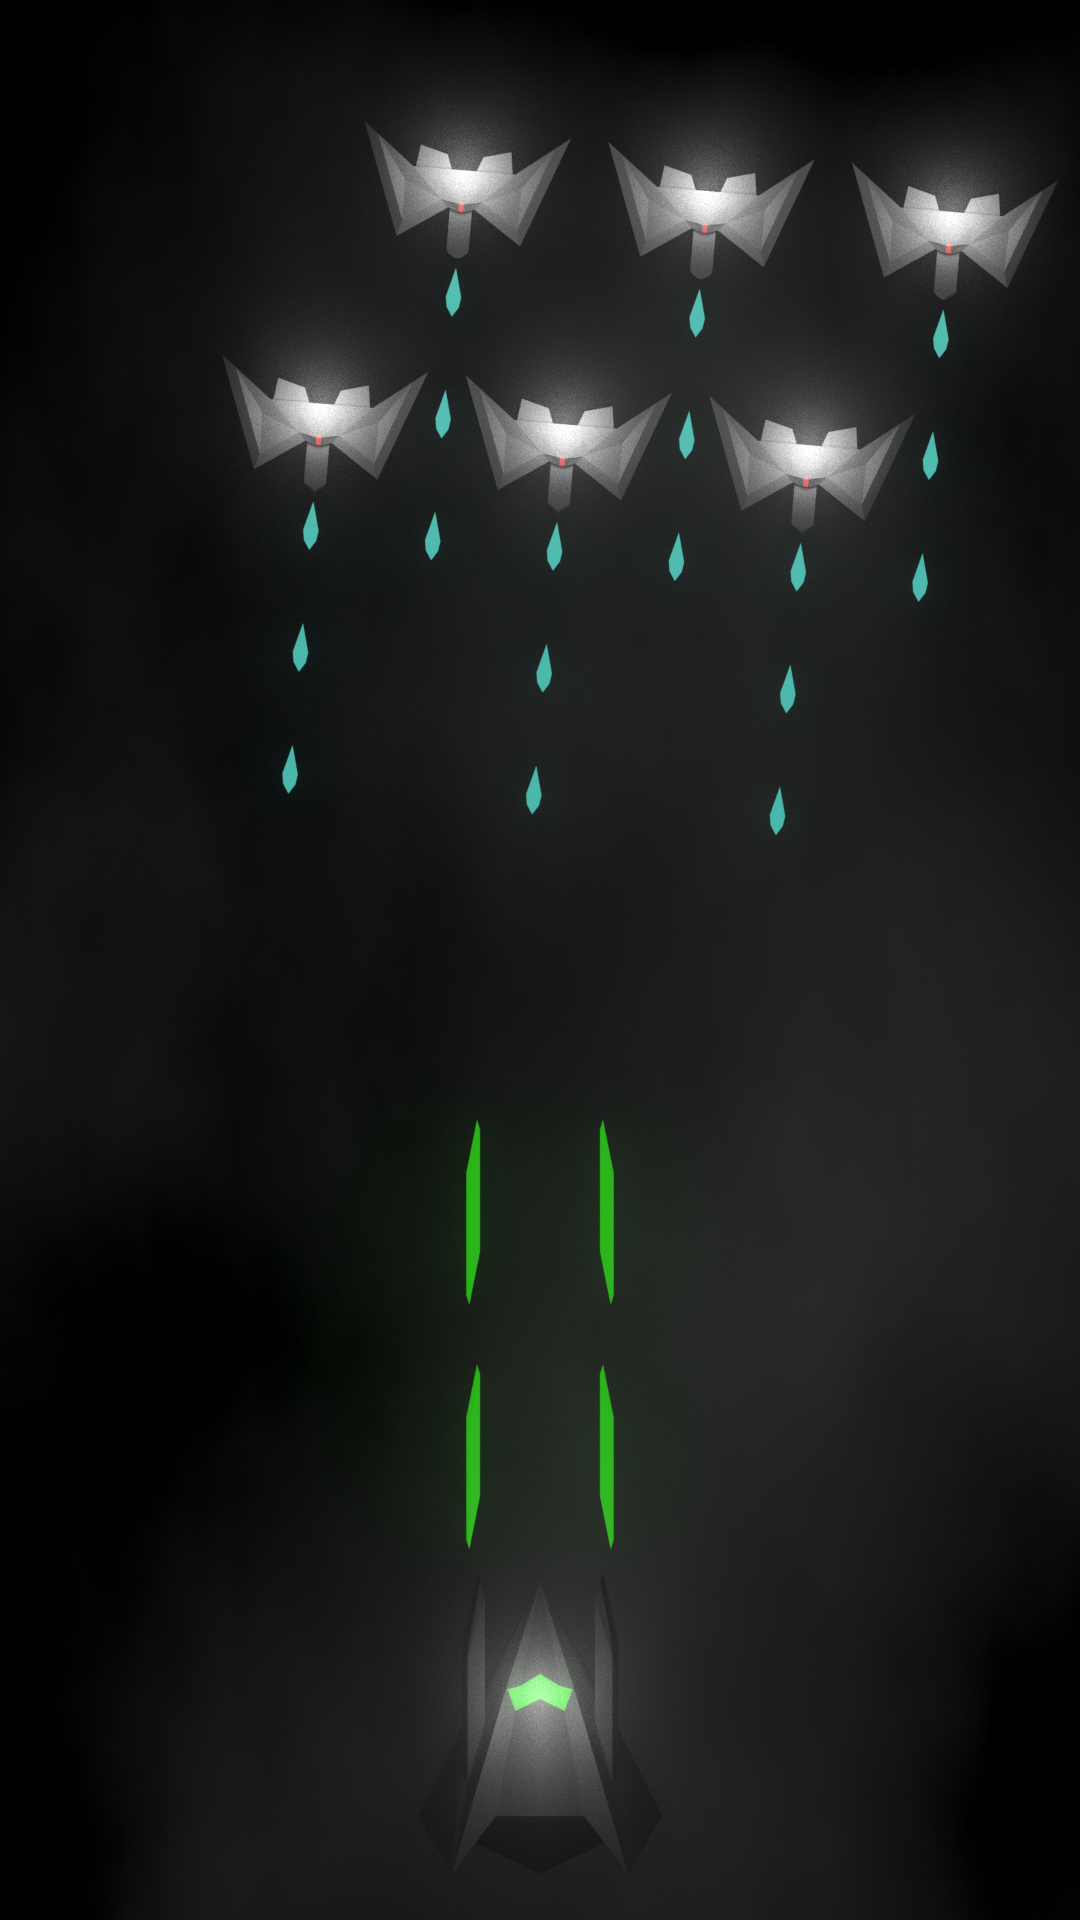
\includegraphics[width=.3\columnwidth]{mockup-01.png}
  \caption[\textit{Cybersky}]{\textit{Cybersky} Mockup Render}
\end{figure}

In terms of feel, the game should be responsive in how the controls work, with a simple input system utilising the touch-screen. The proposed control method involves having an area at the bottom of the screen where the player can swipe or tap to have the ship move horizontally. Vertical movement is not planned as this may be overly complicated for the style of game. This being said, more testing is needed. The scene wireframe in Figure 2 should illustrate this control method.

\begin{figure}[!h]
  \centering
  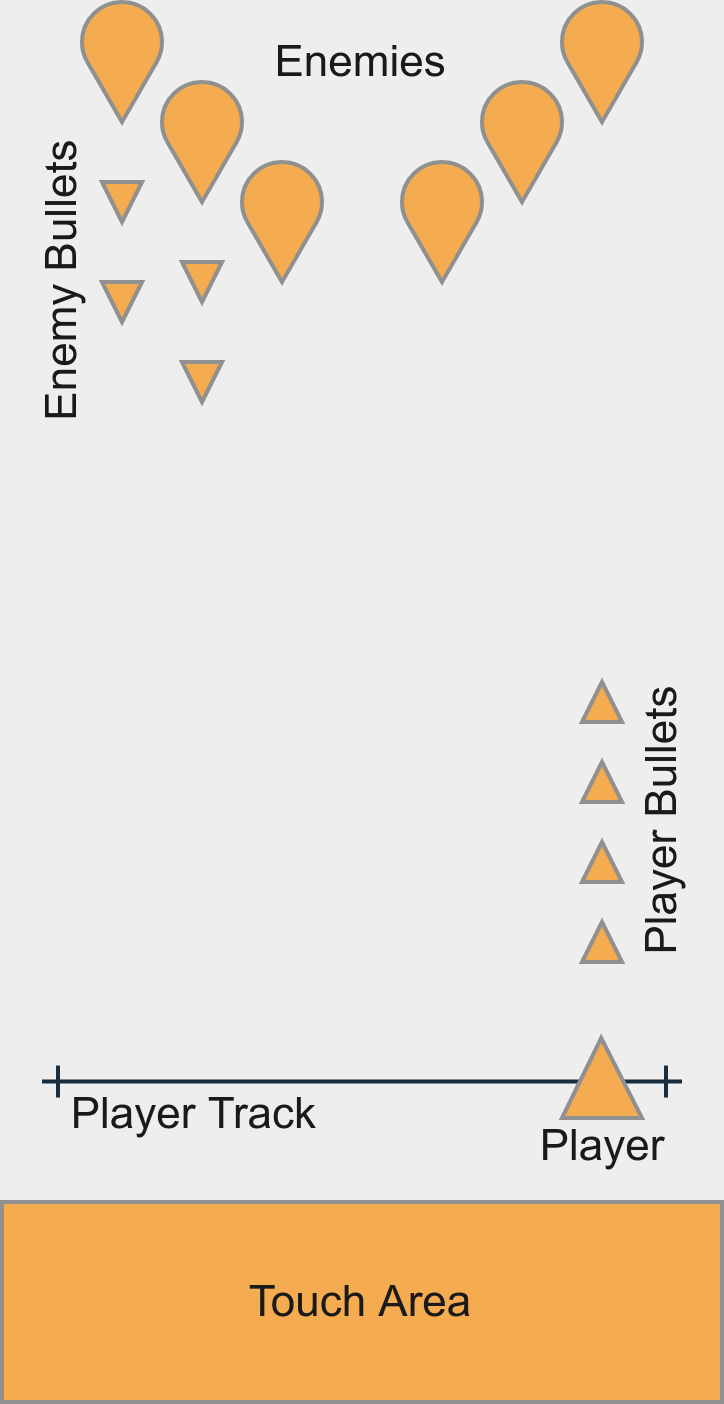
\includegraphics[width=.3\columnwidth]{concept1.png}
  \caption[\textit{Cybersky}]{\textit{Cybersky} Scene Wireframe}
\end{figure}

Not included in this wireframe is the philosophies that could control player movement; whether the ship snaps to the point without any speed limit, whether it moves to the point with a maximum speed, or whether there's two dimensional movement will depend entirely on playtesting and further conceptualisation.

\begin{quote}
  How does this support the desired player’s experience?
\end{quote}

This method of control affects the experience in multiple ways:

\begin{itemize}
  \item The control system is intended to be accessible and simplistic, allowing for entry level gamers to pick up and play.
  \item Additionally, the control system should allow for high level players to accurately and easily move around obstacles.
\end{itemize}

These two together allow for a high skill ceiling and a low skill floor, which fits with the target audiences of the game. As for the visual style, simplistic and yet visually detailed 3D design affords a lot of artistic freedom without much of a hardware limitation; this makes the game more accessible, and lets the environment and object design heavily impact the narrative.

\subsection{Narrative}

Briefly describe the game world and any narrative in player-relevant terms (as presented to the player)

\subsection{Platform(s) and Technology}

Tablet or phone?

2D, 2.5D, or 3D?

Do you use hardware-specific mobile features such as touch screen, location sensing, web connectivity, motion sensing, Bluetooth, WiFi?

\section{
  Game Mechanics
 }

\subsection{Game Rules}

What are the rules that define the game world and the gameplay?

\subsection{Core Loops}

How do game objects and the player’s actions form loops?

Why is this engaging? How does this support the player’s goals?

What emergent results do you expect/hope to see?

If F2P, where are the monetisation points?

\subsection{Objectives and Progression}

How does the player move through the game, literally and figuratively, from tutorial to end?

What are their short-term and long-term goals and rewards (explicit or implicit)?

How do these support the game concept, style, and player-fantasy?

\subsection{Control Schemes}

\subsubsection{Touch}

\subsubsection{Controller}

\printbibliography

\end{document}
